\section{Architecture, contracts, and extending}\label{sec:architecture}

This part is for the day you change the machinery itself -- or wonder why
it is shaped the way it is.

\subsection{The layer map}

% Deliberately plain TikZ: rectangles and labels only. tikz arrives via
% tcolorbox's [most] libraries, so no extra package is loaded for this.
\begin{center}
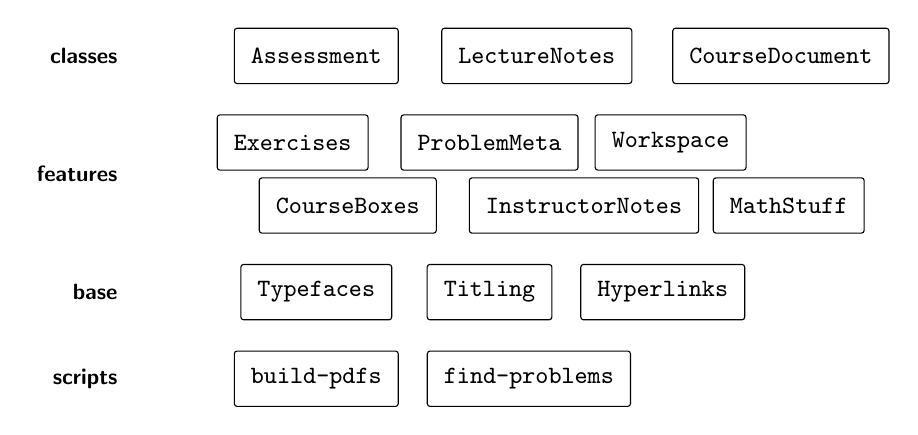
\begin{tikzpicture}[
    box/.style={draw, rounded corners=1pt, minimum height=2em,
                inner xsep=6pt, font=\small\ttfamily},
    band/.style={font=\footnotesize\sffamily\bfseries, anchor=east},
  ]
  % Row 1: the classes
  \node[band] at (-0.6, 3.1) {classes};
  \node[box] at (1.8, 3.1) {Assessment};
  \node[box] at (4.6, 3.1) {LectureNotes};
  \node[box] at (7.7, 3.1) {CourseDocument};
  % Rows 2-3: the feature packages (two rows so nothing crowds)
  \node[band] at (-0.6, 1.6) {features};
  \node[box] at (1.5, 2.0) {Exercises};
  \node[box] at (4.0, 2.0) {ProblemMeta};
  \node[box] at (6.3, 2.0) {Workspace};
  \node[box] at (2.2, 1.2) {CourseBoxes};
  \node[box] at (5.2, 1.2) {InstructorNotes};
  \node[box] at (7.8, 1.2) {MathStuff};
  % Row 4: the base
  \node[band] at (-0.6, 0.1) {base};
  \node[box] at (1.8, 0.1) {Typefaces};
  \node[box] at (4.0, 0.1) {Titling};
  \node[box] at (6.2, 0.1) {Hyperlinks};
  % Alongside: the scripts
  \node[band] at (-0.6, -1.0) {scripts};
  \node[box] at (1.8, -1.0) {build-pdfs};
  \node[box] at (4.5, -1.0) {find-problems};
\end{tikzpicture}
\end{center}

Classes pick from the features; every class stands on the base
(Assessment skips Titling and CourseBoxes; CourseDocument skips the
exercise stack). The scripts sit beside the LaTeX entirely:
\file{build-pdfs} drives latexmk and injects layer flags;
\file{find-problems} reads problem files off disk.

The honest description of the packages' relationship: \emph{not
independent, but coupled through narrow, documented contracts}. Each
package works alone or under a foreign class; where two need each other,
the seam is one macro with a fallback, or a hook with a plain default --
never a hard cross-dependency. The rest of this section documents those
seams.

\subsection{The load-order contract}\label{sec:load-order}

One ordering rule underlies every class, and Typefaces owns it:

\begin{enumerate}
  \item \textbf{amsmath before amsthm, and newtxmath loads amsthm.}
    Typefaces loads amsmath first, then newtxmath with its
    \texttt{amsthm} option -- the one point in newtxmath's load where
    amsthm can arrive in the right order. Consequently \emph{nothing else
    may load amsmath or amsthm} -- and tcolorbox drags amsmath in, which
    is why every tcolorbox-using package must come after Typefaces.
  \item \textbf{The guards enforce it.} MathStuff, CourseBoxes and
    InstructorNotes each open with a check (newtxmath or amsthm loaded?)
    and stop with a clear \cs{PackageError} naming Typefaces as the fix
    -- instead of the cryptic downstream error you would otherwise chase.
  \item \textbf{\texttt{dvipsnames} must reach xcolor first.} A class
    passes the option with \cs{PassOptionsToPackage} before anything
    loads xcolor, since xcolor's options are fixed by whoever loads it
    first.
  \item \textbf{hyperref loads last, via \cs{AtEndPreamble}.} hyperref
    patches much of LaTeX; packages loaded after it can silently undo
    those patches. Hyperlinks defers it past everything the
    \emph{document} loads too -- which \cs{AtEndPreamble} gives and
    \cs{AtEndOfClass} would not.
  \item \textbf{parskip before titlesec} (see the gotchas below for the
    failure mode).
\end{enumerate}

In practice: load Typefaces, then the feature packages, and let
Hyperlinks worry about hyperref -- the order this manual's own preamble
uses.

\subsection{Presentation hooks and narrow couplings}\label{sec:hooks}

The recurring pattern: a shared package provides the \emph{mechanism} and
a plain default look; the consuming class restyles by
\cs{renewcommand}-ing named hooks. Bookkeeping stays in the mechanism, so
no restyle can corrupt it. The instances:

\begin{itemize}
  \item \textbf{Problem headings.} A problem file names no label; the
    class does -- \cs{ProblemLabelWord}, \cs{ProblemHeadingFormat} and
    friends (section~\ref{sec:ref-exercises}) turn one environment into
    ``Problem 7.'', margin-hung ``Q7'', or a run-in ``Example.''
  \item \textbf{The label-word routing.} LectureNotes sets
    \cs{ProblemLabelWord} to read \emph{through}
    \cs{NotesProblemLabelWord}, while Assessment sets it literally to
    ``Q'' -- so a \file{course-vocab.tex} shared by both can retune the
    notes noun with no risk of renaming exam questions.
  \item \textbf{Titles and links.} \cs{TitleColor}, \cs{TitleStamp},
    \cs{LinkColor}, \cs{UrlColor}: plain defaults in the base packages,
    coloured only by CourseDocument. \cs{TitleColor} is a \emph{style}
    hook, not a colour name, precisely so Titling needs no xcolor.
  \item \textbf{\cs{WSZeroHeight}.} Exercises and InstructorNotes route
    their boxes through Workspace's overlay seam -- but each carries an
    \cs{AtBeginDocument} \cs{providecommand} identity fallback, so
    without Workspace the boxes simply render solid. One macro is the
    entire coupling.
  \item \textbf{The \cs{ProblemMeta} stub.} Exercises provides a
    swallow-the-block fallback so the essential package never depends on
    the nice-to-have one.
\end{itemize}

When you add machinery, keep the shape: mechanism $+$ default in the
shared file, look in the class, seams as single \cs{providecommand}-style
macros.

\subsection{Layers and views}

Content visibility is organised as \emph{layers}, each owned by one
package and gated by one flag: solutions and hints (Exercises),
instructor notes (InstructorNotes), the projector variant (LectureNotes).
A \emph{view} is a bundle of layers with a name and a PDF suffix, and
\file{build-pdfs} materialises it by injecting the layer definitions
before \cs{documentclass} is read (\cs{ifdefined} checks in the packages
pick them up -- no class option at any call site). The \env{instructor}
view is the maximal bundle; there is deliberately no marker tier -- the
instructor copy is the staff copy.

The overlay contract (section~\ref{sec:overlay}) is what makes the
layer model safe: turning layers on cannot move a page break, so every
view of a document is page-for-page the same paper.

\subsection{Extending the vocabulary}\label{sec:extending}

\subsubsection*{Declared numbers, and why not counters}

A theorem quoted from the course text must carry \emph{the text's}
number, but notes include only some items, so the sequence legitimately
skips. A LaTeX counter \emph{computes} numbers; a textbook number is an
external fact being \emph{mirrored} -- data, not a computation. Fighting
counters to replay someone else's sequence (scattered \cs{setcounter}s)
yields off-by-one edits and silent drift.

The mechanism that makes declaring cheap is worth recording so nobody
rediscovers it: \cs{label} never reads a counter -- it records whatever
\cs{@currentlabel} holds. So the box environments are \emph{unnumbered}
amsthm environments (\cs{newtheorem*}); the factory sets
\cs{@currentlabel} to the declared number and adds \cs{phantomsection}
for a distinct link anchor. \cs{ref} then resolves to the declared
number, and an edition change costs one token per theorem. (The same
trick, sentinel-valued, is why a stray \cs{label} on an aside prints
\texttt{[unlabelled aside]} instead of silently grabbing the section
number.)

\subsubsection*{course-vocab.tex}

The shared machinery draws a deliberate line: vocabulary every text has
(theorem, definition, \dots) and the author's own asides ship in
CourseBoxes; vocabulary \emph{specific to one text} (APEX's ``Key
Idea'', a geometry text's ``Axiom'') is declared per course, in a small
\file{course-vocab.tex} at the repo root:

\begin{manexsource}
\ifdefined\NewTextResult
  \NewTextResult[cbnote]{keyidea}{Key Idea}{cb/note}
\fi
% \renewcommand{\NotesProblemLabelWord}{Exercise}
\end{manexsource}

Masters \cs{input} it in the preamble (\cs{newtheorem} must run before
the document starts). The \cs{ifdefined} guard is what lets \emph{one}
vocab file serve every master: an Assessment document loads no
CourseBoxes, skips the factory calls, and still picks up non-box
overrides like the notes noun.

To restyle course-wide, prefer the named extension points -- the
\env{cb/*} tcolorbox styles and \env{cb*} head styles
(section~\ref{sec:ref-courseboxes}) -- over per-environment edits.

\subsubsection*{Why the exercise system is homegrown}

The obvious alternative was xsim. A usage audit of the predecessor
course showed only a narrow slice in use: numbered problem/solution
environments, a solutions toggle, points, simple layouts. The one
genuinely hard xsim feature -- \emph{body capture}, writing every
exercise out for replay elsewhere (collected solutions, exercise lists,
random pools) -- was used nowhere, and the toolkit's model is
conditional-inline (a gated \env{solution} in place), never
capture-and-replay. So the homemade system has no hidden cliff ahead:
the cliff is on a path it does not walk, and everything it does need
composes from LaTeX primitives. The trade is owning $\sim$200
understandable lines instead of vendoring $\sim$5{,}800 lines of expl3.
(No maintained alternative package exists; \file{exam.cls} is a class,
architecturally unusable inside three classes.)

\subsection{Silent-failure gotchas}\label{sec:gotchas}

The failure modes that do \emph{not} error -- collected from every
corner of the toolkit, worth a skim before debugging anything odd:

\begin{itemize}
  \item \textbf{parskip's patches fail via \cs{typeout} only.} parskip
    compensates titlesec and the TOC for paragraph skips by patching
    internals at load time; after a titlesec/amsthm upgrade a failed
    patch prints only \texttt{Couldn't patch ...} in the log. Grep for
    it: \texttt{grep "Couldn't patch" *.log}.
  \item \textbf{A reflowed \cs{ProblemMeta} block still compiles} -- and
    silently vanishes from \file{find-problems}
    (section~\ref{sec:problemmeta}).
  \item \textbf{\texttt{[5, hint]} errors} -- the lone-integer points
    shorthand works only alone; write \texttt{[points=5, hint]}.
  \item \textbf{Points are integers}; \texttt{points=2.5} errors at the
    accumulator.
  \item \textbf{\cs{printtotalpoints} and ``Page $N$ of $M$'' print
    \texttt{??} on a clean first pass} -- two-pass values; latexmk's
    rerun settles them.
  \item \textbf{\cs{label} a \env{problemgroup} inside it}, before the
    first part -- after \cs{end} it catches the last part's ``$N$(c)''.
  \item \textbf{\texttt{[unlabelled aside]} in output is the designed
    loud failure} of labelling an aside -- delete the \cs{label}.
  \item \textbf{An overlay box overprinting the content below it} is the
    leave-more-room alarm (section~\ref{sec:overlay}) -- grow the
    workspace.
  \item \textbf{\texttt{[hint]} on a hint-less file warns} rather than
    errors -- the import asked to force a hint that does not exist.
  \item \textbf{A paragraph right after \cs{FreshPage} that opens with a
    literal \texttt{[}} can be swallowed by its optional-argument scan --
    leave a blank line after \cs{FreshPage} (as you naturally would).
  \item \textbf{A \cs{workspace} at the very top of a page is discarded}
    like any top-of-page glue -- put content above it, or use
    \cs{workspace*}.
\end{itemize}

\subsection{Decoupling checklist}

The machinery still carries a little scaffolding from the course it was
built in; a final decoupling pass before any standalone handoff should:
remove the \texttt{TEMPORARY} babel/blindtext loads at the foot of
LectureNotes and CourseDocument (this manual and the demo syllabus lean
on \cs{blindtext} for filler); revisit the hardcoded
\file{~/.cache/latexmk} aux location in \file{build-pdfs}; and retarget
the source comments that still cite the private course-repo notes
(\file{NOTE.md} items) at this manual instead.
